\documentclass[12pt]{article}

%%%%%%%%%%%%%%%%%%%%%%%%%%%%%%%%%%%%%%%%%%%%%%%%%%%%%
% ARQUIVOS RELACIONADOS INCLUIDOS

% pacotes customizados
% Pacotes do relatório
\usepackage[utf8]{inputenc}
\usepackage[T1]{fontenc}
\IfFileExists{lmodern.sty}{\usepackage{lmodern}}{}
% babel em português quando disponível (Overleaf/TeX Live completo)
\IfFileExists{portuges.ldf}{\usepackage[brazil]{babel}}{%
  \usepackage[english]{babel}%
  \addto\captionsenglish{%
    \renewcommand{\figurename}{Figura}\renewcommand{\tablename}{Tabela}%
    \renewcommand{\contentsname}{Sumário}\renewcommand{\listfigurename}{Lista de Figuras}%
    \renewcommand{\listtablename}{Lista de Tabelas}\renewcommand{\refname}{Referências}}}
\usepackage[a4paper,top=25mm,bottom=25mm,left=30mm,right=20mm]{geometry}
\usepackage{amsmath,amssymb}
\usepackage{graphicx}
\usepackage{float}
\usepackage{booktabs}
\usepackage{multirow}
\usepackage{tabularx}
\usepackage{array}
\usepackage[table]{xcolor}
\usepackage{caption}
\usepackage{subcaption}
\usepackage{setspace}
\usepackage{indentfirst}
\usepackage{fancyhdr}
\IfFileExists{lmodern.sty}{\usepackage{microtype}}{\usepackage[expansion=false]{microtype}}
\IfFileExists{siunitx.sty}{\usepackage[output-decimal-marker={,},group-separator={.},per-mode=symbol]{siunitx}}{}
\usepackage[hidelinks]{hyperref}
% nomes do \autoref em português
\AtBeginDocument{%
  \def\figureautorefname{Figura}\def\tableautorefname{Tabela}%
  \def\sectionautorefname{Seção}\def\subsectionautorefname{Seção}%
  \def\subsubsectionautorefname{Seção}\def\equationautorefname{Equação}}
\onehalfspacing
\captionsetup{font=small,labelfont=bf}
\setlength{\headheight}{15pt}
\setlength{\emergencystretch}{3em}


% comandos customizados
\makeatletter
% Parâmetros do documento (mesma interface do template dos relatórios)
\newcommand{\titulo}[1]{\gdef\@titulo{#1}}
\newcommand{\subtitulo}[1]{\gdef\@subtitulo{#1}}
\newcommand{\descricao}[1]{\gdef\@descricao{#1}}
\newcommand{\autores}[1]{\gdef\@autores{#1}}
\newcommand{\departamento}[1]{\gdef\@departamento{#1}}
\newcommand{\professor}[1]{\gdef\@professor{#1}}
\newcommand{\disciplina}[1]{\gdef\@disciplina{#1}}
\newcommand{\turma}[1]{\gdef\@turma{#1}}
\newcommand{\data}[1]{\gdef\@data{#1}}
% Campo a preencher antes da entrega (aparece em vermelho no PDF)
\newcommand{\pendente}[1]{\textcolor{red}{[#1]}}
% Figura que só é incluída se o arquivo existir em imgs/;
% caso contrário, desenha um quadro indicando o arquivo esperado.
% \figuraopcional{arquivo}{rótulo}{legenda}{o que a figura deve mostrar}
\newcommand{\figuraopcional}[4]{%
  \begin{figure}[H]\centering
  \IfFileExists{imgs/#1}{\includegraphics[width=0.9\linewidth]{imgs/#1}}%
  {\fbox{\parbox[c][4.5cm][c]{0.85\linewidth}{\centering\small
     \textcolor{red}{Inserir aqui: \texttt{imgs/#1}}\\[2mm]#4}}}%
  \caption{#3}\label{fig:#2}\end{figure}}
\newcommand{\figura}[3][0.85]{%
  \begin{figure}[H]\centering\includegraphics[width=#1\linewidth]{imgs/#2}
  \caption{#3}\label{fig:#2}\end{figure}}
\makeatother


%%%%%%%%%%%%%%%%%%%%%%%%%%%%%%%%%%%%%%%%%%%%%%%%%%%%%
% PARAMETROS DO DOCUMENTO

% titulo do documento
\titulo{Controle Lateral do Carrinho}

% subtitulo do documento
\subtitulo{Controladores On-off e Stanley com Referência Obtida por Visão Computacional}

% adicione a descricao do trabalho que aparece na contra-capa
\descricao{Relatório técnico apresentado como requisito de avaliação da disciplina Fundamentos de Veículos Autônomos da Universidade Federal de Minas Gerais. O estudo contempla o projeto de dois controladores laterais para o carrinho, um controlador on-off com histerese e o controlador Stanley, avaliados no CoppeliaSim inicialmente em trajetórias geométricas (reta, círculo e oito) e, em seguida, seguindo a linha amarela da pista detectada pela câmera embarcada. Em todos os ensaios a velocidade é regulada pelo controlador PI longitudinal desenvolvido na Parte 1. Também é avaliado o quão rápido cada controlador completa o percurso sem capotar ou perder a pista. Por fim, o controlador Stanley é testado no veículo físico, seguindo uma faixa amarela no piso.}

% nome dos autores. Separe-os por '\\'
\autores{João Henrique Menezes Oliveira -- 2022055122 \\ Lara Strutz Carvalho -- 2023039325 \\ Leonardo Carlos Maciel Corrêa -- 2020035817 \\ Rian Rero Lopes Jericó Vieira -- 2023039473}

% departamento
\departamento{Departamento de Engenharia Eletrônica (DELT)}

% professor
\professor{Armando Alves Neto e Leonardo Amaral Mozelli}

% codigo da disciplina
\disciplina{ENG075}

% turma
\turma{TFVA}

% data do documento
\data{\today}


%%%%%%%%%%%%%%%%%%%%%%%%%%%%%%%%%%%%%%%%%%%%%%%%%%%%%
% INICIO DO DOCUMENTO
\begin{document}

\makeatletter
\begin{titlepage}
\centering
\IfFileExists{resources/logo.png}{\includegraphics[width=0.28\linewidth]{resources/logo.png}\par\vspace{8mm}}{}
{\large UNIVERSIDADE FEDERAL DE MINAS GERAIS\par}
{\large Escola de Engenharia\par}
{\large \@departamento\par}
\vfill
{\Huge\bfseries \@titulo\par}\vspace{6mm}
{\Large \@subtitulo\par}
\vfill
{\large \@autores\par}
\vfill
{\large \@data\par}
\end{titlepage}

\begin{titlepage}
\centering
{\large \@autores\par}
\vfill
{\Large\bfseries \@titulo\par}\vspace{4mm}{\large \@subtitulo\par}
\vfill
\hfill\begin{minipage}{0.55\linewidth}\small\singlespacing
\@descricao\par\vspace{5mm}
\textbf{Professores:} \@professor\\
\textbf{Disciplina:} \@disciplina\quad\textbf{Turma:} \@turma
\end{minipage}
\vfill
{\large Belo Horizonte\par\@data\par}
\end{titlepage}
\makeatother
\pagestyle{fancy}\fancyhf{}\fancyhead[R]{\small\nouppercase{\leftmark}}\fancyfoot[C]{\thepage}
\renewcommand{\headrulewidth}{0.4pt}
\tableofcontents
\newpage


%%%%%%%%%%%%%%%%%%%%%%%%%%%%%%%%%%%%%%%%%%%%%%%%%%%%%
% *COLOQUE SUAS SEÇÕES TEXTUAIS AQUI
\section{Introdução}\label{sec:introducao}

Na Parte 1 foi desenvolvido o controle longitudinal do carrinho \cite{mozelli2025controlelongitudinal}. Para percorrer trajetórias curvilíneas, é necessário também um controle lateral, que atua no esterçamento das rodas dianteiras para manter o veículo sobre um caminho desejado. Neste trabalho foram implementados e comparados dois controladores laterais vistos em sala \cite{mozelli2025controlelateral}: um controlador \textit{on-off}, que comanda o esterçamento em três níveis ($-\delta_{on}$, $0$, $+\delta_{on}$) a partir de um erro de orientação, e o controlador Stanley \cite{thrun2006stanley,hoffmann2007stanley}, que calcula o esterçamento de forma contínua a partir dos erros de orientação e lateral no eixo dianteiro. Em todos os ensaios, a velocidade é mantida pelo PI longitudinal da Parte 1, sem alterações.

O desenvolvimento foi feito no CoppeliaSim \cite{coppeliasim}, na cena \texttt{simulador\_cones.ttt}, cuja pista tem uma linha amarela pintada no centro; os cones foram ignorados. Primeiro, os controladores foram testados com referências geométricas (reta, círculo e oito), usando a pose verdadeira do veículo, para avaliar as leis de controle sem erros de percepção. Em seguida, a referência passou a ser estimada somente pela câmera embarcada, por um algoritmo que segmenta a linha amarela e a projeta no chão, e o carrinho percorreu a volta completa da pista ($\approx246\,\mathrm{m}$) com diferentes velocidades, para determinar o quão rápido cada controlador completa o percurso sem capotar ou se perder. Por fim, o Stanley foi testado no carrinho real, seguindo uma faixa amarela no piso. Os códigos estão no repositório do projeto \cite{desgovernai2026}, e o arquivo \texttt{LEIA-ME.txt} descreve como reproduzir cada resultado.

\section{Plataformas e Arquitetura do Sistema}\label{sec:arquitetura}

Os ensaios foram realizados no CoppeliaSim 4.10, na cena \texttt{simulador\_cones.ttt}. A aplicação em Python comunica-se com o simulador pela API remota ZMQ em modo síncrono: a cada passo de $50\,\mathrm{ms}$, o mesmo período do PI de velocidade, são lidos os estados e a imagem, calculados os comandos e avançada a simulação. O esterçamento é aplicado por \texttt{car.setSteer()}, que converte o ângulo do modelo bicicleta nos ângulos das duas rodas por Ackermann. Com $|\delta|\le20^\circ$ e $L=0{,}302\,\mathrm{m}$, o menor raio de curva é $L/\tan20^\circ\approx0{,}83\,\mathrm{m}$. Na cena, um comando positivo vira para a direita; os controladores usam a convenção usual (positivo para a esquerda) e o sinal é invertido apenas na aplicação.

A câmera é perspectiva, de $600\times400$ pixels e abertura de $60^\circ$, montada a $\approx0{,}35\,\mathrm{m}$ do chão e inclinada $\approx10^\circ$ para baixo. A borda inferior da imagem corresponde a um ponto $\approx0{,}5\,\mathrm{m}$ à frente do eixo dianteiro, ou seja, a linha nunca é vista sob o ponto em que o erro lateral é definido. A \autoref{tab:parametros-laterais} resume os parâmetros. Os controladores, as referências geométricas e a cadeia de visão estão em \texttt{fva\_car/lateral.py} e \texttt{fva\_car/trajetorias.py}; o laço de ensaio, em \texttt{controle\_lateral.py}.

\begin{table}[ht]
    \centering
    \caption{Parâmetros do veículo simulado e dos controladores laterais.}
    \label{tab:parametros-laterais}
    \small
    \begin{tabular}{lc}
        \hline
        Parâmetro & Valor \\
        \hline
        Período de controle e de aquisição da imagem & $50\,\mathrm{ms}$ \\
        Esterçamento máximo / taxa máxima (ambos os controladores) & $20^\circ$ / $60^\circ/\mathrm{s}$ \\
        On-off: amplitude $\delta_{on}$ / histerese $h_{on}$, $h_{off}$ & $15^\circ$ / $3^\circ$, $1^\circ$ \\
        On-off: distância de antecipação $L_d$ & $0{,}8\,\mathrm{m}$ \\
        Stanley: ganho $k$ / suavização $v_s$ & $1{,}5\,\mathrm{s^{-1}}$ / $0{,}3\,\mathrm{m/s}$ \\
        Controle longitudinal (Parte 1) & PI, $k_p=4$, $k_i=2$ \\
        \hline
    \end{tabular}
\end{table}

\section{Metodologia}\label{sec:metodologia}

\subsection{Erros de seguimento}

Com o modelo cinemático de bicicleta ($\dot\psi = v\tan\delta/L$), os dois controladores usam erros definidos no centro do eixo dianteiro $p_f$ \cite{hoffmann2007stanley}. Sendo $P$ o ponto da referência mais próximo de $p_f$, $\psi_r$ a direção da sua tangente e $\hat n_r$ a normal à esquerda,
\begin{equation}
e_y = (P - p_f)\cdot \hat n_r, \qquad e_\psi = \psi_r - \psi .
\end{equation}
Assim, $e_y>0$ indica referência à esquerda e $e_\psi>0$ indica que o veículo precisa girar para a esquerda.

\subsection{Controlador on-off}

Um on-off que atuasse apenas sobre $e_\psi$ deixaria o veículo paralelo à referência, sem eliminar o deslocamento lateral. Por isso, a referência de orientação foi definida como a direção de um ponto da referência a uma distância $L_d=0{,}8\,\mathrm{m}$ adiante de $P$, ao longo da tangente. No referencial do veículo, esse ponto está exatamente no ângulo
\begin{equation}
e = e_\psi + \arctan\left(e_y/L_d\right),
\label{eq:erro-onoff}
\end{equation}
que é o erro usado pelo on-off. O esterçamento assume três níveis, com histerese:
\begin{equation}
\delta_k = +\delta_{on}\ \text{se}\ e>h_{on};\quad -\delta_{on}\ \text{se}\ e<-h_{on};\quad 0\ \text{se}\ |e|<h_{off};\quad \delta_{k-1}\ \text{nos demais casos}.
\end{equation}
O nível zero evita oscilação contínua entre os batentes nas retas. A amplitude $\delta_{on}$ deve superar o esterçamento de regime $\arctan(L\kappa)$ da curva mais fechada, mas, quanto maior, maior o ciclo-limite; o valor de $15^\circ$ foi escolhido pelos ensaios de sensibilidade (\autoref{sec:resultados}). O comando passa pelo mesmo limitador de taxa do Stanley.

\subsection{Controlador Stanley}

O Stanley \cite{thrun2006stanley,hoffmann2007stanley,snider2009steering} soma a correção da orientação a um termo não linear do erro lateral:
\begin{equation}
\delta = \operatorname{sat}_{\pm\delta_{\max}}\left[e_\psi + \arctan\left(\frac{k\,e_y}{v_s+|v|}\right)\right].
\label{eq:stanley}
\end{equation}
Para erros pequenos e sem saturação, $\dot e_y \approx -k|v|\,e_y/(v_s+|v|)$: convergência exponencial com constante de tempo próxima de $1/k$, aproximadamente independente da velocidade. Com $k=1{,}5\,\mathrm{s^{-1}}$ e $v=1\,\mathrm{m/s}$, ela vale $\approx0{,}87\,\mathrm{s}$.

\subsection{Referências geométricas}

Na primeira etapa, os erros foram calculados com a pose verdadeira do simulador em relação a: uma \textbf{reta} de $28\,\mathrm{m}$ deslocada $0{,}5\,\mathrm{m}$ para a esquerda da pose inicial (convergência a partir de um erro inicial); um \textbf{círculo} de raio $3\,\mathrm{m}$ tangente à pose inicial (curvatura constante); e um \textbf{oito} formado por dois círculos de $3\,\mathrm{m}$ percorridos em sentidos opostos, em cujo cruzamento a curvatura salta de $+1/3$ para $-1/3\,\mathrm{m^{-1}}$. Os ensaios foram feitos numa região plana e sem cones, para a qual o carrinho é reposicionado (a cena não é salva), com $v_{ref}=1{,}0$ e $2{,}0\,\mathrm{m/s}$.

\subsection{Estimação da referência por visão computacional}\label{sec:visao}

Na segunda etapa, $e_y$ e $e_\psi$ são estimados somente a partir da imagem, a cada passo:
\begin{enumerate}
    \item \textbf{Segmentação}: conversão para HSV e seleção de $40^\circ\le H\le75^\circ$, $S\ge0{,}4$, $V\ge0{,}2$, o que elimina o asfalto e as faixas brancas.
    \item \textbf{Centro da linha}: a máscara é percorrida de baixo para cima; em cada linha da imagem é escolhido o segmento amarelo mais próximo do centro anterior, descartando saltos maiores que $20\%$ da largura (outros trechos da linha ao fundo).
    \item \textbf{Projeção no chão}: cada centro gera um raio pelo modelo \textit{pinhole}, intersectado com o plano da pista.
    \item \textbf{Memória curta}: pontos dos últimos $3\,\mathrm{s}$ a até $3\,\mathrm{m}$ do eixo dianteiro são mantidos, para cobrir a região cega; ela só é usada se houve detecção nos últimos $0{,}3\,\mathrm{s}$.
    \item \textbf{Ajuste local}: no referencial do veículo, o trecho até $\approx1{,}2\,\mathrm{m}$ à frente é ajustado por uma parábola, com rejeição de pontos atípicos; o ponto mais próximo do eixo dianteiro fornece $e_y$, $e_\psi$ e a curvatura $\kappa$. Em curvas fechadas, um arco de circunferência substitui a parábola quando tem menor resíduo, pois extrapola melhor até o eixo.
\end{enumerate}
A medida é rejeitada com menos de seis pontos, extensão menor que $0{,}3\,\mathrm{m}$ ou resíduo acima de $12\,\mathrm{cm}$. Numa falha curta, o último esterçamento é mantido por até $0{,}4\,\mathrm{s}$; depois, a velocidade de referência é zerada. A projeção e a memória usam a pose da câmera dada pelo simulador (equivalente a odometria ideal), mas os erros enviados ao controle vêm apenas dos pixels detectados.

\subsection{Ensaios na pista e critérios de avaliação}

Na pista, $v_{ref}$ foi mantida constante ($0{,}5$ a $2{,}5\,\mathrm{m/s}$, o máximo do veículo) para isolar o efeito da velocidade. Também foi testada a redução nas curvas, $v_{ref}^{*}=\min\{v_{ref},\max[0{,}5;\ \min(\sqrt{a_{lat}/|\kappa|},\ v_{ref}/(1+2|e_y|+|e_\psi|))]\}$, com $a_{lat}=1{,}5\,\mathrm{m/s^2}$ e $\kappa$ estimada pela câmera. Cada ensaio parte da pose original da cena e termina ao completar a volta (retorno a menos de $1\,\mathrm{m}$ do início) ou numa falha: inclinação da carroceria acima de $45^\circ$ (capotamento), distância maior que $1\,\mathrm{m}$ da linha (saída da pista) ou mais de $1\,\mathrm{s}$ sem detecção (perdido).

Como o erro estimado pela câmera não é independente, foi calculado também um erro verdadeiro: a distância do eixo dianteiro ao esqueleto da linha amarela extraído da textura da pista (pixels de $1{,}8\,\mathrm{cm}$), usado apenas na avaliação e nos critérios de término. As métricas desconsideram os primeiros $5\,\mathrm{s}$.

\section{Resultados}\label{sec:resultados}

Os valores desta seção estão em \texttt{metricas.csv}, gerado a partir dos registros pelo script \texttt{figuras\_lateral.py}.

\subsection{Referências geométricas}

A \autoref{fig:geo-trajetorias} mostra o caminho do eixo dianteiro a $1{,}0\,\mathrm{m/s}$ e a \autoref{tab:geo} resume as métricas. Todos os ensaios foram concluídos.

\begin{figure}[ht]
    \centering
    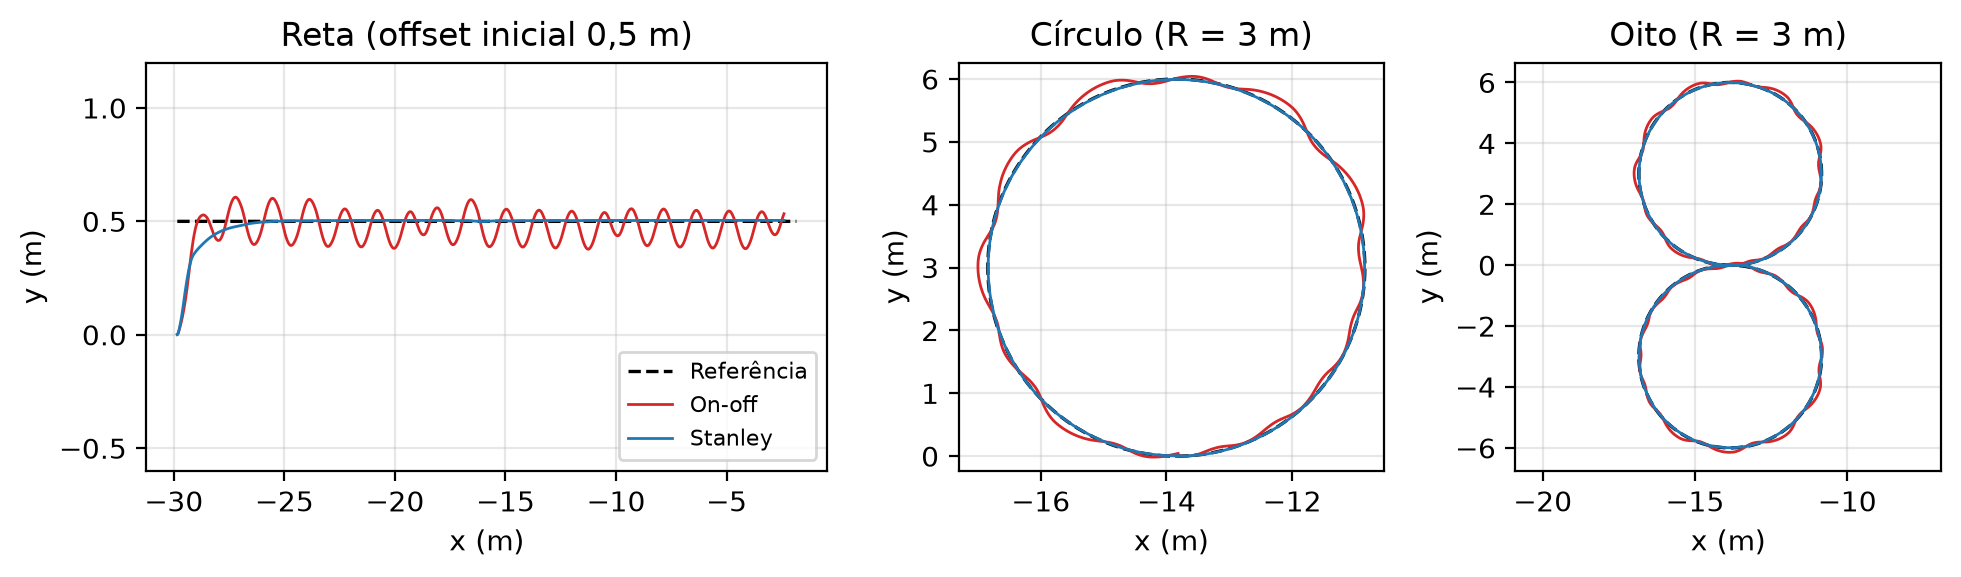
\includegraphics[width=\textwidth]{imgs/geo_trajetorias.png}
    \caption{Trajetória do eixo dianteiro com referências geométricas a $1{,}0\,\mathrm{m/s}$. Os erros são calculados com a pose verdadeira do simulador.}
    \label{fig:geo-trajetorias}
\end{figure}

\begin{table}[ht]
    \centering
    \caption{Erro lateral nas referências geométricas (após $5\,\mathrm{s}$): RMS e máximo, RMS da taxa de esterçamento e frequência de comutação do on-off.}
    \label{tab:geo}
    \small
    \setlength{\tabcolsep}{4pt}
    \begin{tabular}{llccccccc}
        \hline
        & & \multicolumn{4}{c}{On-off} & \multicolumn{3}{c}{Stanley} \\
        Referência & $v_{ref}$ & RMS & Máx. & $\dot\delta_{\mathrm{RMS}}$ & Comut. & RMS & Máx. & $\dot\delta_{\mathrm{RMS}}$ \\
        & $(\mathrm{m/s})$ & $(\mathrm{cm})$ & $(\mathrm{cm})$ & $(^\circ/\mathrm{s})$ & $(\mathrm{s^{-1}})$ & $(\mathrm{cm})$ & $(\mathrm{cm})$ & $(^\circ/\mathrm{s})$ \\
        \hline
        Reta    & $1{,}0$ & $6{,}5$  & $12{,}3$ & $48$ & $2{,}0$ & $0{,}37$ & $0{,}44$ & $11$ \\
                & $2{,}0$ & $28{,}2$ & $45{,}4$ & $43$ & $1{,}1$ & $0{,}20$ & $0{,}37$ & $15$ \\
        Círculo & $1{,}0$ & $8{,}3$  & $15{,}7$ & $48$ & $2{,}4$ & $0{,}45$ & $0{,}71$ & $4$ \\
                & $2{,}0$ & $36{,}4$ & $68{,}1$ & $44$ & $1{,}6$ & $0{,}39$ & $0{,}85$ & $3$ \\
        Oito    & $1{,}0$ & $7{,}7$  & $16{,}1$ & $48$ & $2{,}5$ & $0{,}47$ & $1{,}35$ & $5$ \\
                & $2{,}0$ & $38{,}1$ & $70{,}8$ & $43$ & $1{,}3$ & $0{,}73$ & $4{,}00$ & $7$ \\
        \hline
    \end{tabular}
\end{table}

O on-off mantém o veículo sobre as referências, mas em ciclo-limite: o esterçamento alterna continuamente e o erro oscila com amplitude de $12$--$16\,\mathrm{cm}$ a $1{,}0\,\mathrm{m/s}$. Ao dobrar a velocidade, o erro RMS aumenta de quatro a cinco vezes. O Stanley tem erro RMS abaixo de $1\,\mathrm{cm}$ em todos os casos e taxa de esterçamento de 3 a 15 vezes menor.

No oito (\autoref{fig:geo-oito}), o Stanley converge para $\approx5{,}7^\circ$, o valor de regime $\arctan(L/R)=5{,}75^\circ$, e o salto de curvatura no cruzamento ($t\approx19\,\mathrm{s}$) gera um pico de apenas $1{,}4\,\mathrm{cm}$. O on-off não tem esse nível e obtém a curvatura média alternando entre $+15^\circ$ e $0$ ou $-15^\circ$, o que gera a oscilação.

\begin{figure}[ht]
    \centering
    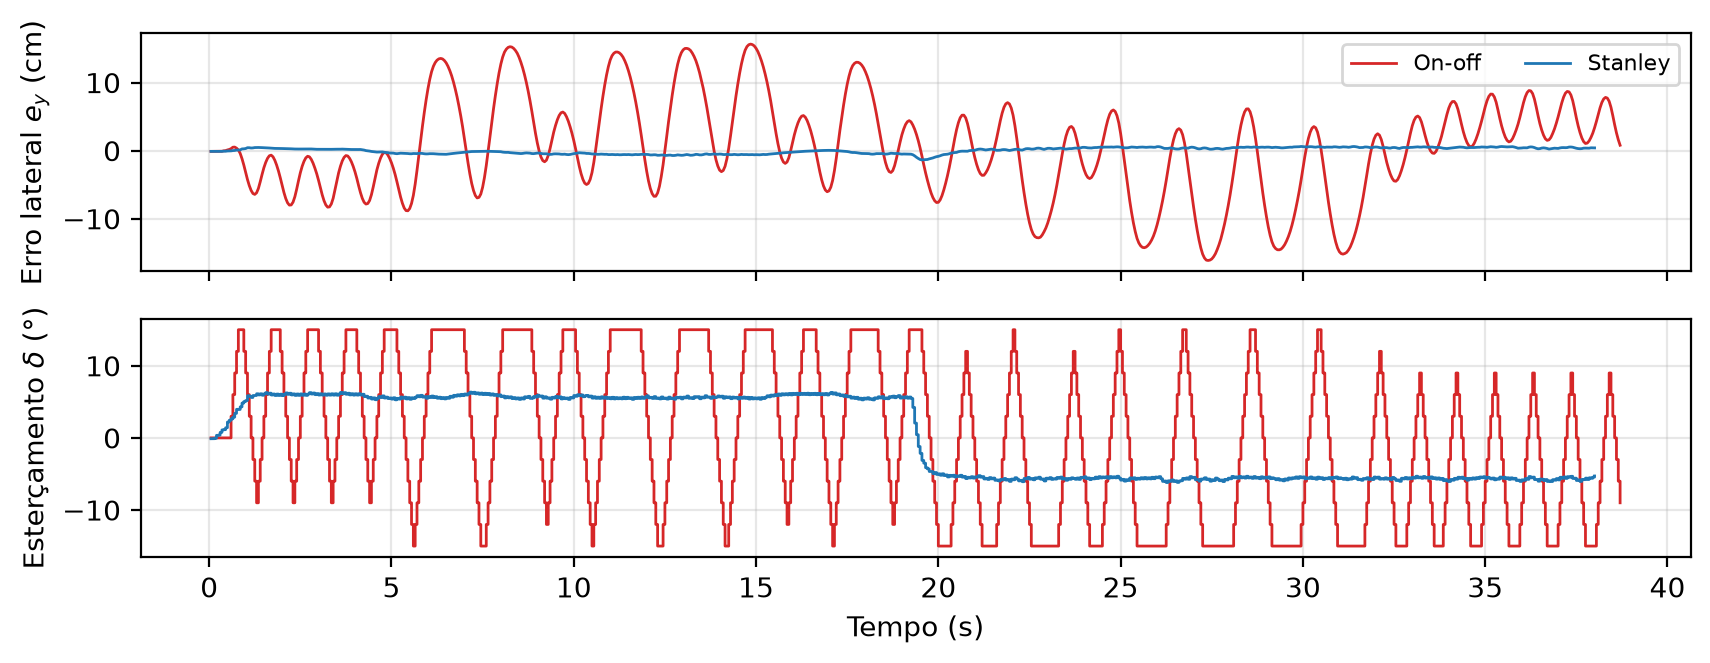
\includegraphics[width=\textwidth]{imgs/geo_oito_tempo.png}
    \caption{Erro lateral e esterçamento no oito a $1{,}0\,\mathrm{m/s}$. A troca de sentido da curva ocorre em $t\approx19\,\mathrm{s}$.}
    \label{fig:geo-oito}
\end{figure}

\textbf{Sensibilidade.} No on-off, o ciclo-limite cresce com a amplitude: no oito, o erro RMS foi de $4{,}1$, $7{,}7$ e $15{,}4\,\mathrm{cm}$ para $\delta_{on}=8$, $15$ e $20^\circ$. O valor de $8^\circ$ basta no oito, que exige $5{,}7^\circ$, mas não nas curvas mais fechadas da pista (\autoref{sec:res-visao}). No Stanley, partindo de $0{,}5\,\mathrm{m}$ de erro na reta, $k=0{,}5\,\mathrm{s^{-1}}$ converge lentamente (constante de tempo $\approx2{,}6\,\mathrm{s}$), $k=1{,}5\,\mathrm{s^{-1}}$ converge em $\approx4\,\mathrm{s}$ sem sobressinal e $k=5\,\mathrm{s^{-1}}$ apresenta sobressinal de $21\,\mathrm{cm}$, causado pela saturação em $20^\circ$ e pelo limite de taxa, ausentes da análise linearizada. Foi mantido $k=1{,}5\,\mathrm{s^{-1}}$.

\subsection{Seguimento da linha amarela pela câmera}\label{sec:res-visao}

A \autoref{fig:visao-pipeline} ilustra a cadeia de visão numa curva: os pontos projetados ficam a mais de $0{,}5\,\mathrm{m}$ do eixo dianteiro, e o ajuste local é extrapolado até ele. Nas voltas, a curvatura estimada teve percentil 99 de $\approx0{,}7\,\mathrm{m^{-1}}$ (raio de $1{,}4\,\mathrm{m}$), que exige $\approx12^\circ$ de esterçamento de regime.

\begin{figure}[ht]
    \centering
    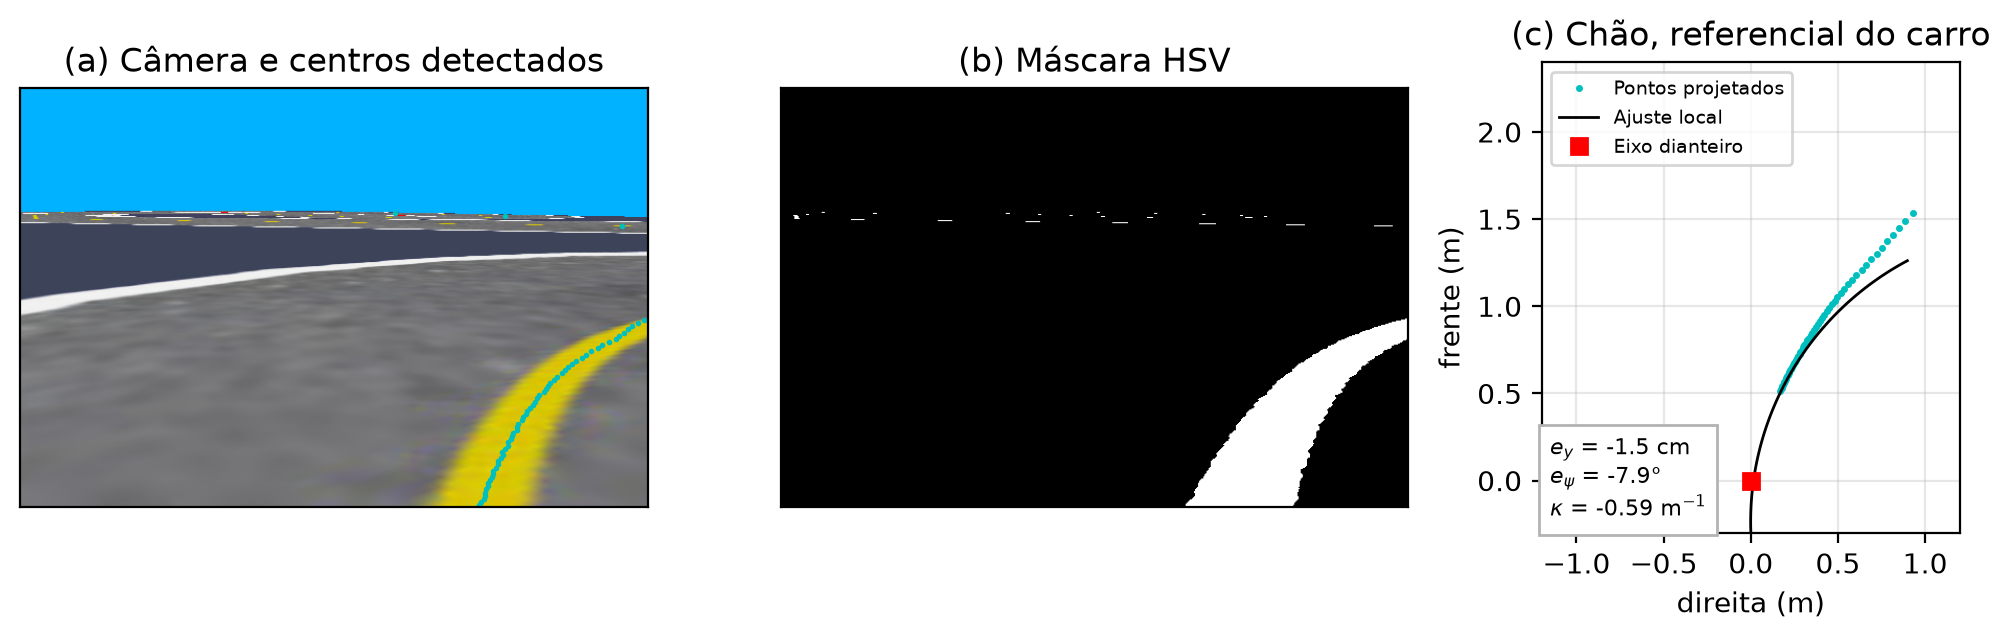
\includegraphics[width=\textwidth]{imgs/visao_pipeline.png}
    \caption{Cadeia de visão em um único quadro (sem memória): (a) imagem da câmera e centros da linha; (b) máscara HSV; (c) pontos projetados no chão, ajuste local e erros resultantes.}
    \label{fig:visao-pipeline}
\end{figure}

A \autoref{tab:visao} resume as voltas ($\approx246\,\mathrm{m}$) com velocidade constante. O Stanley completou o percurso em todas as velocidades, inclusive na máxima do veículo, $2{,}5\,\mathrm{m/s}$, em $99{,}7\,\mathrm{s}$. O on-off só completou a volta a $0{,}5$ e $0{,}75\,\mathrm{m/s}$; a partir de $1{,}0\,\mathrm{m/s}$ falhou cada vez mais cedo.

\begin{table}[ht]
    \centering
    \caption{Volta completa com referência visual e $v_{ref}$ constante. Erros verdadeiros medidos em relação à linha da textura, após $5\,\mathrm{s}$; a última coluna é o RMS do erro estimado pela câmera.}
    \label{tab:visao}
    \small
    \setlength{\tabcolsep}{3.5pt}
    \begin{tabular}{llcccccc}
        \hline
        Controlador & $v_{ref}$ & Resultado & Tempo & RMS & P95 & Máx. & RMS visual \\
        & $(\mathrm{m/s})$ & & $(\mathrm{s})$ & $(\mathrm{cm})$ & $(\mathrm{cm})$ & $(\mathrm{cm})$ & $(\mathrm{cm})$ \\
        \hline
        On-off  & $0{,}5$  & volta completa & $488{,}9$ & $2{,}8$ & $6{,}0$ & $10{,}6$ & $3{,}1$ \\
                & $0{,}75$ & volta completa & $328{,}3$ & $3{,}4$ & $6{,}3$ & $10{,}4$ & $3{,}9$ \\
                & $1{,}0$  & perdeu a linha ($163\,\mathrm{m}$) & $161{,}2$ & $7{,}0$ & $12{,}3$ & $48{,}5$ & $6{,}9$ \\
                & $1{,}5$  & perdeu a linha ($91\,\mathrm{m}$) & $60{,}7$ & $12{,}8$ & $21{,}9$ & $52{,}9$ & $12{,}0$ \\
                & $2{,}0$  & saiu da pista ($53\,\mathrm{m}$) & $27{,}1$ & $26{,}1$ & $42{,}3$ & $101$ & $23{,}3$ \\
                & $2{,}5$  & saiu da pista ($21\,\mathrm{m}$) & $9{,}7$ & $54{,}0$ & $86{,}6$ & $104$ & $44{,}9$ \\
        \hline
        Stanley & $1{,}0$ & volta completa & $245{,}6$ & $1{,}0$ & $2{,}3$ & $5{,}7$ & $0{,}6$ \\
                & $1{,}5$ & volta completa & $164{,}3$ & $1{,}1$ & $2{,}2$ & $6{,}1$ & $0{,}9$ \\
                & $2{,}0$ & volta completa & $123{,}8$ & $1{,}7$ & $3{,}3$ & $16{,}9$ & $1{,}8$ \\
                & $2{,}5$ & volta completa & $99{,}7$ & $3{,}6$ & $4{,}9$ & $33{,}0$ & $3{,}8$ \\
        \hline
    \end{tabular}
\end{table}

A \autoref{fig:pista} compara os controladores a $1{,}0\,\mathrm{m/s}$. O on-off oscila durante todo o percurso e perde a linha no canto mais fechado, em $(-1{,}5;\ 9{,}4)\,\mathrm{m}$: o comando estava em $-15^\circ$ quando a linha começou a curvar para a esquerda, o erro de orientação chegou a $33^\circ$, acima da meia abertura da câmera ($30^\circ$), e a linha saiu da imagem. Em velocidades maiores a falha ocorre antes; a $2{,}5\,\mathrm{m/s}$, ainda na reta inicial. O Stanley mantém o erro abaixo de $2{,}3\,\mathrm{cm}$ em $95\%$ da volta; os maiores erros ocorrem nos dois cantos vivos da linha.

\begin{figure}[ht]
    \centering
    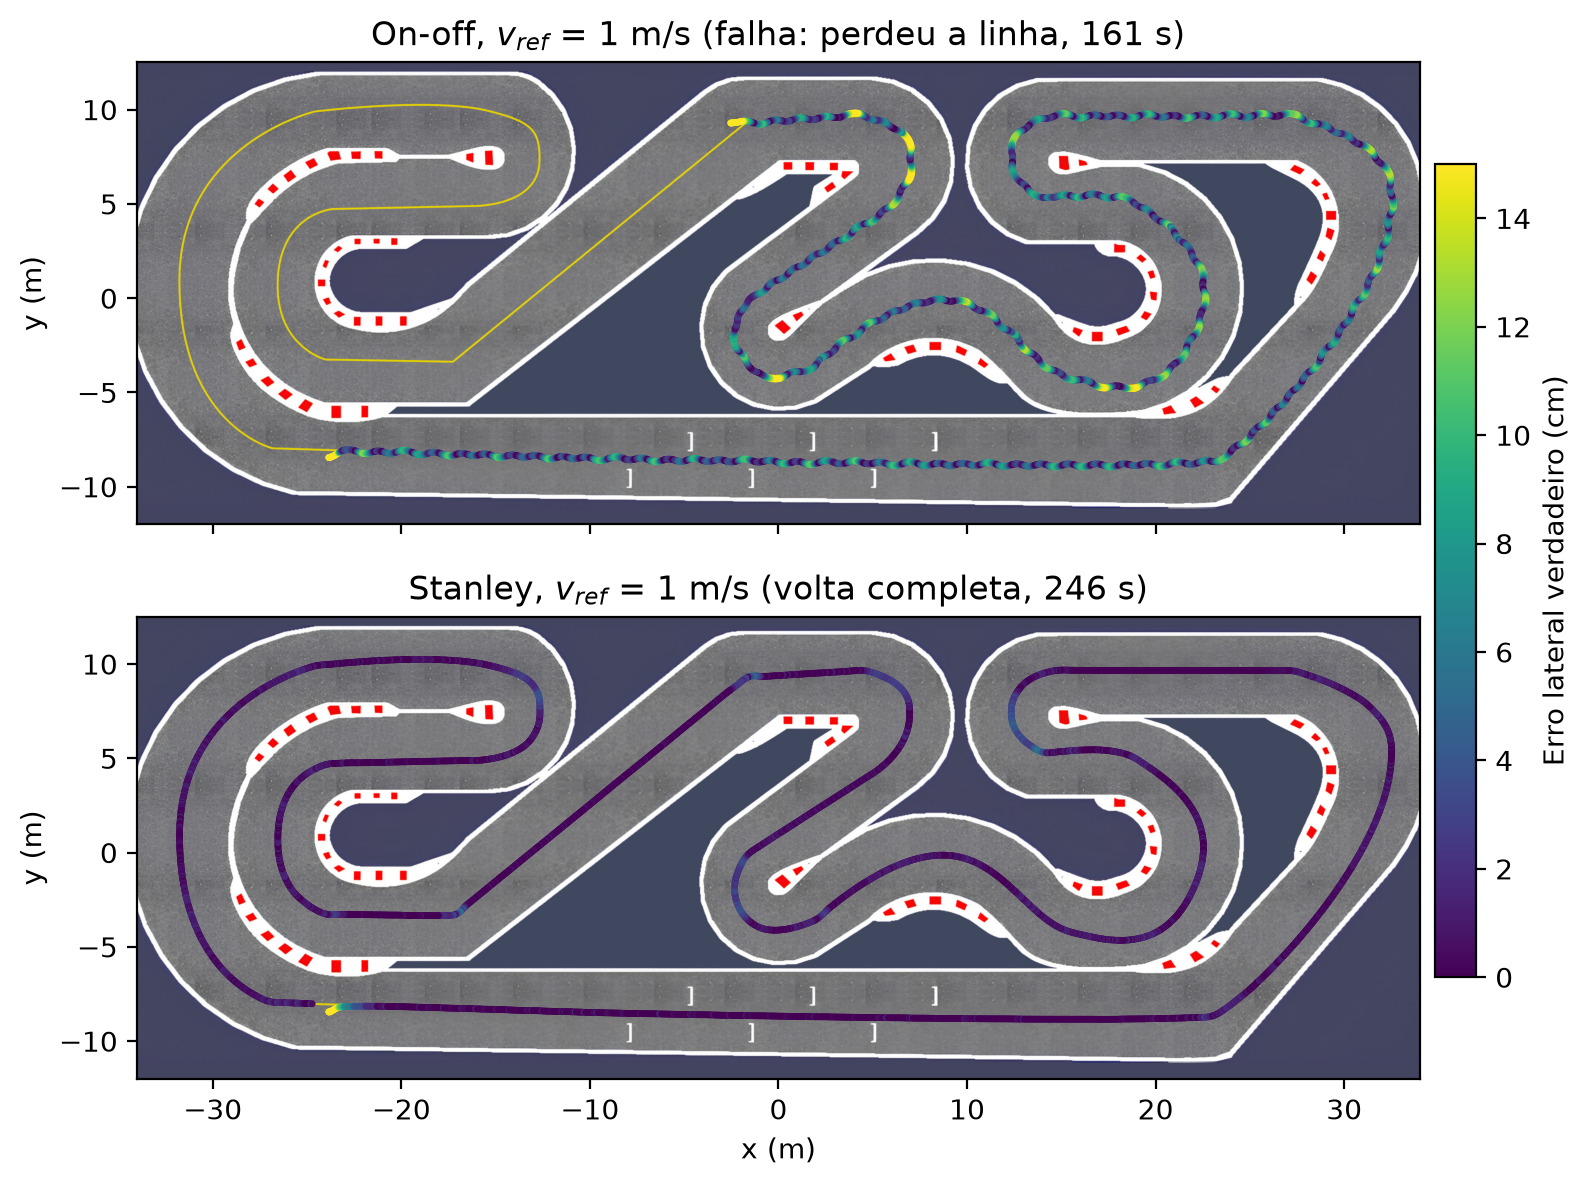
\includegraphics[width=0.88\textwidth]{imgs/pista_1.png}
    \caption{Trajetória do eixo dianteiro sobre a pista a $1{,}0\,\mathrm{m/s}$, colorida pelo erro lateral verdadeiro. O carrinho parte de $(-24;\ -8{,}5)\,\mathrm{m}$ e percorre a pista no sentido anti-horário.}
    \label{fig:pista}
\end{figure}

Com a velocidade, o erro do Stanley cresce sobretudo nesses cantos: a $2{,}5\,\mathrm{m/s}$ o pico foi de $33\,\mathrm{cm}$, com RMS de $3{,}6\,\mathrm{cm}$ e inclinação máxima da carroceria de $9{,}3^\circ$, longe do capotamento. A linha foi detectada em $100\%$ dos passos, e o RMS estimado pela câmera ficou próximo do verdadeiro, indicando que a visão não introduz viés significativo.

\textbf{Redução nas curvas.} Com $v_{ref}=2{,}5\,\mathrm{m/s}$ e redução nas curvas, o Stanley completou a volta em $107{,}9\,\mathrm{s}$ (média de $2{,}28\,\mathrm{m/s}$), só $8\%$ a mais, enquanto o erro RMS caiu de $3{,}6$ para $1{,}8\,\mathrm{cm}$, o pico de $33{,}0$ para $17{,}4\,\mathrm{cm}$ e a inclinação de $9{,}3^\circ$ para $2{,}9^\circ$. O on-off, nas mesmas condições, perdeu a linha após $52\,\mathrm{m}$, pois a oscilação nas retas, em velocidade máxima, já é excessiva.

\textbf{Amplitude do on-off na pista.} Com $\delta_{on}=8^\circ$, o veículo completou a volta a $0{,}5\,\mathrm{m/s}$, mas com pico de $23{,}4\,\mathrm{cm}$ (contra $10{,}6\,\mathrm{cm}$ com $15^\circ$), e a $0{,}75\,\mathrm{m/s}$ perdeu a linha após $178\,\mathrm{m}$, numa curva com curvatura estimada de $1{,}2\,\mathrm{m^{-1}}$. Com $8^\circ$ o menor raio possível é $L/\tan8^\circ=2{,}1\,\mathrm{m}$, o que confirma a escolha de $15^\circ$.

\subsection{Validação no veículo real}\label{sec:res-real}

O Stanley foi testado no carrinho físico, seguindo uma fita amarela no piso de um corredor, com a mesma lei e os mesmos parâmetros do simulador. A faixa é detectada em HSV numa imagem de $320\times240$ pixels e convertida para o chão por uma homografia calibrada com pontos medidos a partir do eixo dianteiro. O controle longitudinal é o PI do veículo real desenvolvido na Parte 1 ($k_p=1$, $k_i=0{,}8$ e \textit{feedforward}). Foram realizados sete ensaios de $30\,\mathrm{s}$; o on-off não foi testado no veículo real.

\begin{table}[ht]
    \centering
    \caption{Ensaios do Stanley no carrinho real. Os erros são estimados pela câmera (não há referência independente) e calculados somente com a faixa detectada.}
    \label{tab:real}
    \small
    \setlength{\tabcolsep}{3.5pt}
    \begin{tabular}{ccccccl}
        \hline
        Ensaio & $v_{ref}$ & Faixa & RMS $e_y$ & Máx. $|e_y|$ & RMS $e_\psi$ & Término \\
        & $(\mathrm{m/s})$ & detectada & $(\mathrm{cm})$ & $(\mathrm{cm})$ & $(^\circ)$ & \\
        \hline
        1 & $0{,}63$ & $99{,}4\%$ & $2{,}1$ & $16{,}3$ & $5{,}4$ & $30\,\mathrm{s}$ completos \\
        2 & $0{,}63$ & $100\%$ & $2{,}6$ & $15{,}9$ & $7{,}7$ & parada por obstáculo ($22\,\mathrm{s}$) \\
        3 & $0{,}63$ & $100\%$ & $2{,}0$ & $4{,}6$ & $5{,}7$ & falha de leitura do encoder ($21\,\mathrm{s}$) \\
        4 & $1{,}29$ & $100\%$ & $5{,}3$ & $9{,}7$ & $5{,}1$ & parada por obstáculo ($8\,\mathrm{s}$) \\
        5 & $0{,}61$ & $71{,}3\%$ & $5{,}3$ & $31{,}0$ & $14{,}2$ & perdas da faixa a partir de $8{,}6\,\mathrm{s}$ \\
        6 & $0{,}63$ & $95{,}5\%$ & $2{,}9$ & $21{,}0$ & $5{,}7$ & $30\,\mathrm{s}$ completos \\
        7 & $0{,}63$ & $99{,}0\%$ & $2{,}6$ & $4{,}8$ & $4{,}7$ & $30\,\mathrm{s}$ completos \\
        \hline
    \end{tabular}
\end{table}

A \autoref{tab:real} resume os ensaios e a \autoref{fig:real} mostra o ensaio 7. Nos ensaios sem interrupções (1, 6 e 7), o RMS do erro estimado ficou entre $2{,}1$ e $2{,}9\,\mathrm{cm}$, da mesma ordem do simulador, e a velocidade acompanhou a referência de $\approx0{,}63\,\mathrm{m/s}$. No ensaio 4, a $1{,}29\,\mathrm{m/s}$, a faixa foi mantida por $8\,\mathrm{s}$ até a parada pelo ultrassom. No ensaio 5, a faixa não foi detectada em $29\%$ das amostras.

Exceto no ensaio 5, os erros médios foram positivos ($e_y\approx+1{,}4$ a $+4{,}4\,\mathrm{cm}$, $e_\psi\approx+3$ a $+5^\circ$) e o esterçamento médio ficou em $6$--$7^\circ$, embora a curvatura estimada da faixa fosse próxima de zero. A informação visual chegou ao controle com idade mediana de $\approx0{,}15\,\mathrm{s}$.

\begin{figure}[ht]
    \centering
    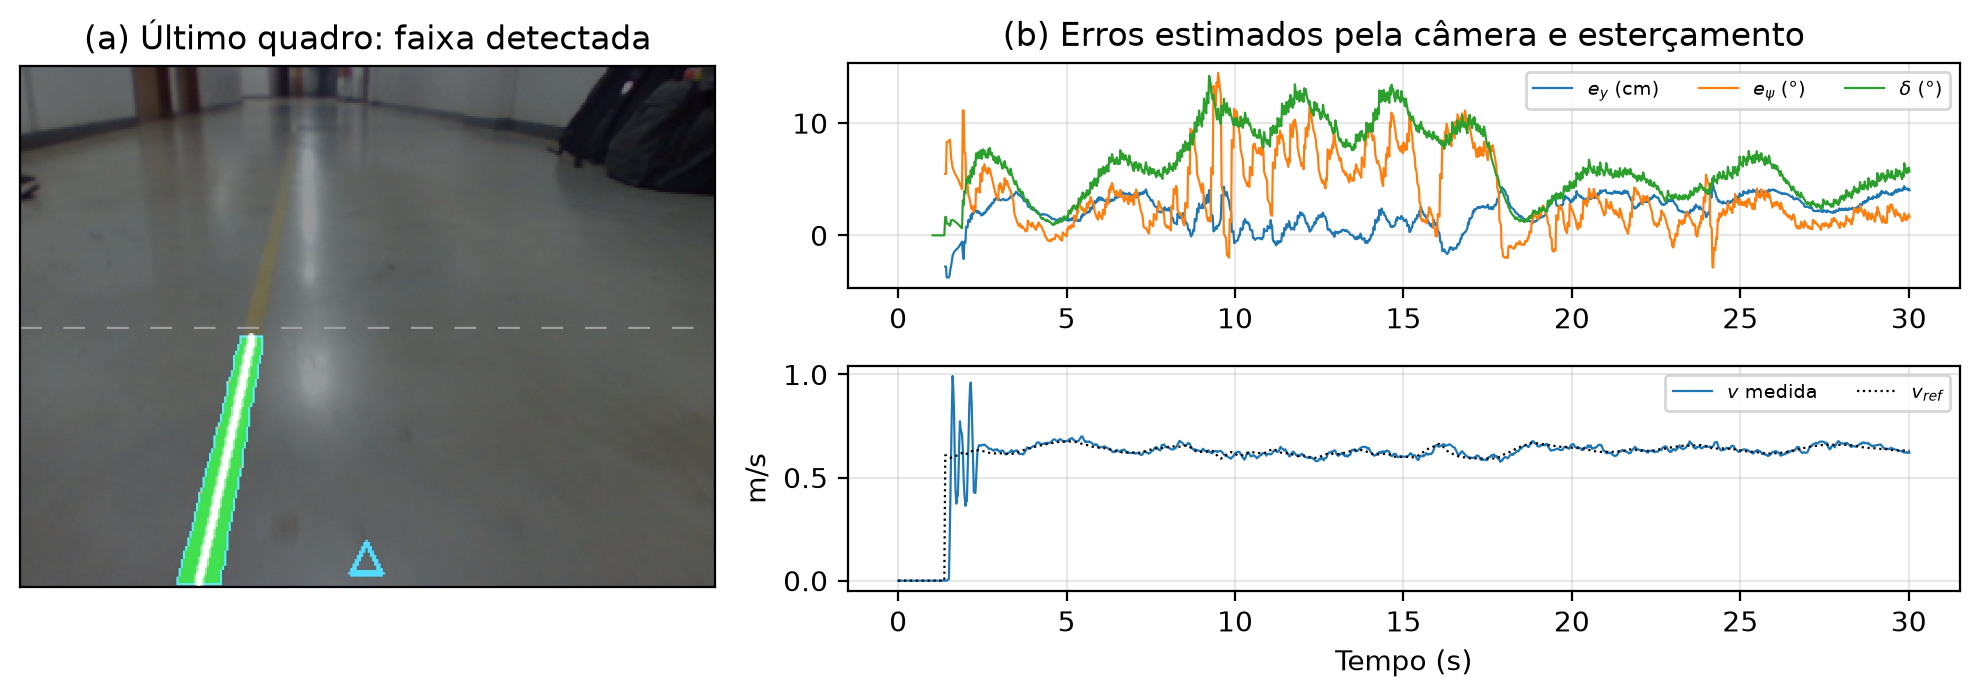
\includegraphics[width=0.92\textwidth]{imgs/real_stanley.png}
    \caption{Ensaio 7 do Stanley no carrinho real: (a) último quadro, com a faixa detectada em verde; (b) erros estimados pela câmera, esterçamento, velocidade e referência.}
    \label{fig:real}
\end{figure}

\section{Discussão}\label{sec:discussao}

\textbf{On-off.} Sem um nível igual ao esterçamento de regime de cada curva, o on-off nunca atinge o equilíbrio e o erro descreve um ciclo-limite. Sua amplitude depende do tempo de reversão do comando (histerese, período de $50\,\mathrm{ms}$ e limite de taxa, $\approx0{,}5\,\mathrm{s}$ de $+15^\circ$ a $-15^\circ$), durante o qual o veículo se desloca lateralmente a uma taxa proporcional a $v$. Por isso o erro cresce com a velocidade e diverge a $2{,}5\,\mathrm{m/s}$ ainda na reta. Com a câmera, que enxerga apenas $\pm30^\circ$ e não vê os primeiros $0{,}5\,\mathrm{m}$ à frente do eixo, uma oscilação que coincide com uma curva fechada leva a linha para fora da imagem. A amplitude $\delta_{on}$ impõe um compromisso entre o tamanho do ciclo-limite e o raio mínimo de curva, $L/\tan\delta_{on}$. A distância de antecipação $L_d$ foi essencial: sem o termo $\arctan(e_y/L_d)$, o on-off corrigiria apenas a orientação.

\textbf{Stanley.} Em regime, o termo $e_\psi$ fornece o esterçamento necessário para a curvatura, e o erro fica na faixa de milímetros com referências ideais e de $1$--$4\,\mathrm{cm}$ com a câmera. Os maiores erros com visão aparecem nos cantos vivos da linha pintada: o ajuste local, feito com pontos a mais de $0{,}5\,\mathrm{m}$ à frente, é extrapolado até o eixo e não representa a quina, e o atuador limitado em taxa não reproduz o salto de esterçamento. Por isso o pico cresce com a velocidade (de $6$ para $33\,\mathrm{cm}$) enquanto o RMS cresce pouco, e a redução de velocidade nas curvas diminui o pico pela metade com pequeno custo no tempo de volta.

\textbf{Do simulador para o veículo real.} A mesma lei, com os mesmos ganhos, manteve o carrinho real sobre a faixa com erro estimado de $2$--$3\,\mathrm{cm}$ a $\approx0{,}6\,\mathrm{m/s}$. Os erros médios positivos, com esterçamento médio de $6$--$7^\circ$ numa faixa praticamente reta, indicam um viés sistemático, como desalinhamento mecânico da direção ou erro de guinada na calibração da câmera. Como o Stanley não possui ação integral, um desvio constante só é compensado com erro permanente; uma correção de \textit{trim} ou um termo integral pequeno eliminariam esse viés. O veículo real ainda apresenta atraso visual de $\approx0{,}15\,\mathrm{s}$, perdas de detecção e falhas de outros subsistemas (encoder, ultrassom) que interromperam ensaios. O on-off não foi testado no veículo real; pela simulação, ele exigiria velocidades baixas.

\textbf{Limitações.} No simulador, a projeção e a memória usam a pose da câmera fornecida pela cena, o que equivale a odometria ideal, e a segmentação HSV foi avaliada com iluminação constante. O erro verdadeiro tem resolução de $1{,}8\,\mathrm{cm}$, de modo que valores abaixo de $\approx1\,\mathrm{cm}$ estão próximos do limite da referência, e cada condição foi ensaiada uma única vez. No veículo real não há referência independente: os erros são estimados pela própria câmera, a odometria (encoder e modelo cinemático, sem IMU) acumula deriva e não foi usada como medida, e apenas trechos de $30\,\mathrm{s}$ foram percorridos.

\section{Conclusão}\label{sec:conclusao}

Foram desenvolvidos e comparados dois controladores laterais, um on-off de três níveis com histerese e o Stanley, integrados ao PI de velocidade da Parte 1. Com referências geométricas, o Stanley obteve erros RMS abaixo de $1\,\mathrm{cm}$, enquanto o on-off apresentou ciclo-limite com erro RMS de $6$--$8\,\mathrm{cm}$ a $1{,}0\,\mathrm{m/s}$ e de $28$--$38\,\mathrm{cm}$ a $2{,}0\,\mathrm{m/s}$.

Com a referência obtida pela câmera (segmentação HSV, projeção no chão e ajuste local), o Stanley completou a volta de $246\,\mathrm{m}$ em todas as velocidades, inclusive em $2{,}5\,\mathrm{m/s}$, em $99{,}7\,\mathrm{s}$ e com erro verdadeiro RMS de $3{,}6\,\mathrm{cm}$; a redução de velocidade nas curvas custou $8\%$ no tempo e reduziu o erro pela metade. O on-off completou a volta apenas até $0{,}75\,\mathrm{m/s}$ ($328\,\mathrm{s}$) e, acima disso, perdeu a linha ou saiu da pista. Nenhum ensaio terminou em capotamento.

No veículo real, o Stanley com os ganhos do simulador seguiu a faixa a $\approx0{,}63\,\mathrm{m/s}$ com erro estimado de $2$--$3\,\mathrm{cm}$, mas revelou um viés de esterçamento a ser corrigido. Conclui-se que o Stanley é claramente superior para percorrer a pista com rapidez e precisão, enquanto o on-off, embora simples, só é adequado em baixa velocidade.


%%%%%%%%%%%%%%%%%%%%%%%%%%%%%%%%%%%%%%%%%%%%%%%%%%%%%

% bibliografia
\nocite{*}
\bibliographystyle{unsrt}
\bibliography{resources/bibliografia}

\end{document}
